\documentclass[a4paper,compress,13pt]{beamer}
\usepackage{wan2i}

\title{WAN2i}%\\ Wide Area Network}
\subtitle{Wide Area Network}
\author[Pierre {\sc Bettens}]{Pierre {\sc Bettens} \\ \small \texttt{pbettens(\`a)heb.be}}
\institute{ÉSI - École Supérieure d'Informatique}
\date{18/09/2012}


\begin{document}

\begin{frame}[fragile]
	\titlepage
\end{frame}


\section{Organisation}

\begin{frame}[fragile]
  \frametitle{Organisation}
Évaluation
\begin{itemize}
	\item \textit{À venir}
\end{itemize}

Supports
\begin{itemize}
	\item Slides
\end{itemize}

Références
	\begin{itemize}
		\item Réseaux 5\raisebox{5pt}{\scriptsize e} édition \\ 
		\textit{Andrew Tanenbaum et David Wetherall}
	\end{itemize}
\end{frame}


\section{Préalables}

\begin{frame}[fragile]
  \frametitle{Préalables}
\begin{center}
	\Huge{\bf\color{blue}Préalables}
\end{center}
\begin{flushright}
  \item Définition
  \item Utilité
\end{flushright}
\end{frame}

\begin{frame}[fragile]
  \frametitle{Préalables}
\textbf{WAN \textit{wide area network}}
\begin{itemize}
	\item Un WAN peut être vu comme une interconnexion de LAN
	\item Ce qui caractérise un WAN, c'est la \textbf{distance} entre les hôtes
	... mais pas seulement
	\begin{itemize}
		\item ce sont des \textbf{personnes différentes} qui gèrent les composants
		\item les routeurs connectent des réseaux de \textbf{technologies différentes}
	\end{itemize}

	\item Deux types de composants
	\begin{itemize}
		\item les lignes de transmission (fil de cuivre, fibre optique, liaison radio, ...)
		\item les équipements de commutation (routers)
	\end{itemize}
\end{itemize}
\end{frame}

\begin{frame}[fragile]
  \frametitle{Préalables}
\textbf{Utilité} \\
Une entreprise veut connecter plusieurs filiales, géographiquement distantes, entre elles
\begin{itemize}
	\item Par le biais de lignes louées
	\item \textit{via} Internet, par le biais de VPN (\textit{virtual private network})
\end{itemize}

Exemples
\begin{itemize}
	\item Internet
	\item Le téléphone
	\item Les réseaux d'entreprise
\end{itemize}
\end{frame}

\section{Rappels réseaux}

\begin{frame}[fragile]
  \frametitle{Rappels réseaux}
\begin{center}
	\Huge{\bf\color{blue}Rappels réseaux}
\end{center}
\begin{flushright}
  \item Préalables
  \item Modèle OSI
  \item Modèle TCP/ IP
  \item Ethernet
\end{flushright}
\end{frame}

\begin{frame}[fragile]
  \frametitle{Rappels réseaux}
{\bf\Large Préalable}

Afin de modéliser le fonctionnement des réseaux, la complexité est décomposée en
\textbf{couches}; chaque couche repose sur la couche inférieure afin d'offrir
des services à la couche supérieure
\begin{itemize}
	\item Modèle OSI
	\item Modèle TCP / IP
	\item Ethernet
\end{itemize}
\end{frame}


\section{Rappels réseaux - Modèle OSI}

\begin{frame}[fragile]
  \frametitle{Rappels réseaux - Modèle OSI}
Le \textbf{modèle OSI} propose un découpage en 7 couches. 
À ces couches sont associés des protocoles que nous n'étudions pas.

\begin{center}
	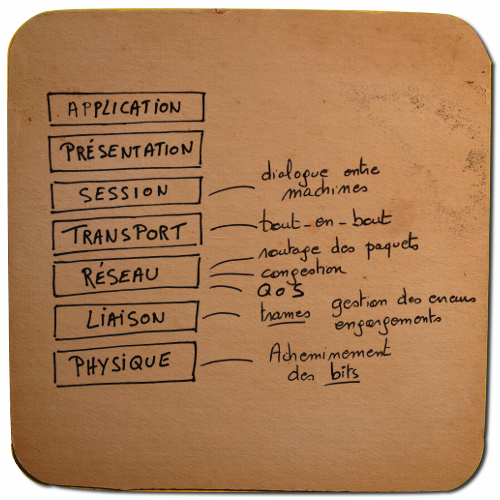
\includegraphics[width=.55\linewidth]{img/modele-osi-500x500.png}
\end{center}
\end{frame}

\begin{frame}[fragile]
  \frametitle{Rappels réseaux - Modèle OSI}
\begin{itemize}
	\item Couche physique (\textit{physical layer})
	\begin{itemize}
		\item Transmission des bits sur le support
		\item Gestion des différents supports; fibre optique, cuivre, onde radio, courant porteur, ...
	\end{itemize}
	\item Couche liaison de données (\textit{data link layer})
	\begin{itemize}
		\item Montrer à la couche \textit{network}, une transmission sans
		erreurs non détectées
		\item Transmet des \textbf{trames} de données
		\item Doit gérer les différences de vitesse entre l'émetteur et le récepteur (engorgement)
	\end{itemize}
	\item Couche réseau (\textit{network layer})
	\begin{itemize}
		\item Transmet de \textbf{paquets} de données
		\item Détermine comment les paquets sont routés d'un point à un autre
		\item Gestion de la congestion et de la qualité de service
	\end{itemize}
\end{itemize}
\end{frame}

\begin{frame}[fragile]
  \frametitle{Rappels réseaux - Modèle OSI}
\begin{itemize}
	\item Couche transport 	(\textit{transport layer})
	\begin{itemize}
		\item Accepte des données de la couche supérieure et les transmet
		\item Veille à la transmission de bout en bout
		\item Autorise différents types de services; point-à-point sans erreur, diffusion à plusieurs destinataires, ...
	\end{itemize}
	\item Couche session (\textit{session layer}
	\begin{itemize}
		\item Permet l'établissement d'une session (dialogue, synchronisation, ...)
	\end{itemize}
	\item Couche présentation (\textit{presentation layer})
	\begin{itemize}
		\item Permet une certaine abstraction des données transmises
	\end{itemize}
	\item Couche application (\textit{application layer})
	\begin{itemize}
		\item Définit les différents protocoles; http, smtp, ftp, ...
	\end{itemize}
\end{itemize}
\end{frame}

\begin{frame}[fragile]
  \frametitle{Rappels réseaux - Modèle OSI}
\begin{center}
	{\Large Nous nous concentrerons sur les couches \\ 
	\textit{physical, data link} et \textit{network}}
\end{center}
\end{frame}


\section{Rappels réseaux - Modède TCP / IP}

\begin{frame}[fragile]
  \frametitle{Rappels réseaux - Modède TCP / IP}
Le \textbf{modèle TCP / IP} propose également un découpage en couches. On s'intéresse particulièrement aux protocoles associés au modèle.

\begin{center}
	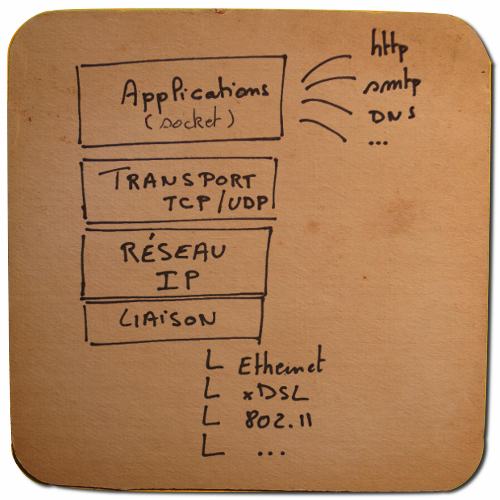
\includegraphics[width=.55\linewidth]{img/modele-tcpip-500x500.png}
\end{center}
\end{frame}

\begin{frame}[fragile]
  \frametitle{Rappels réseaux - Modède TCP / IP}
\begin{itemize}
	\item Interface de liaison
	\begin{itemize}
		\item Permet de faire un lien entre le support physique et l'adresse IP de la machine
		\item Les protocoles associés, ethernet, SONET, xDSL, 802.x
	\end{itemize}
	\item Couche internet (\textit{internet layer})
	\begin{itemize}
		\item Permet l'introduction de paquets sur le réseau ...
		\item ... ces paquets seront acheminés vers l'hôte de destination (même sur un autre réseau)
		\item \textbf{Les} protocoles associés sont \textbf{IP} et ICMP
	\end{itemize}
	\item Couche transport (\textit{transport layer})
	\begin{itemize}
		\item Permet à deux hôtes de communiquer
		\item \textbf{Les} protocoles associés sont \textbf{TCP} et \textbf{UDP}
		\begin{itemize}
			\item TCP, protocole fiable avec connexion assure le contrôle de flux
			\item UDP, protocole non fiable sans connexion
		\end{itemize}
	\end{itemize}
	\item Les applications
\end{itemize}
\end{frame}


\section{Rappels réseaux - Ethernet}

\begin{frame}[fragile]
  \frametitle{Rappels réseaux - Ethernet}
Deux normes proches / confondues; \textbf{802.3} et \textbf{Ethernet}

Distinguer
\begin{itemize}
	\item Ethernet classique
	\begin{itemize}
		\item Débit 3-10 Mbit/s
	\end{itemize}
	\item Ethernet commuté
	\begin{itemize}
		\item Utilisation de commutateurs (\textit{switch})
		\item Débit 100 Mbit/s pour «Fast Ethernet»
		\item Débit 1 Gbit/s pour «Gigabit Ethernet»
		\item Débit 10 Gbit/s
	\end{itemize}
\end{itemize}
\end{frame}

\begin{frame}[fragile]
  \frametitle{Rappels réseaux - Ethernet}
{\large\bf Couche physique}
\begin{itemize}
	\item Jadis, cable coaxial
	\item Paire torsadée
\end{itemize}

{\large\bf Sous couche d'accès au réseau (\textit{Media Access Control})}
\begin{itemize}
	\item Format de la trame Ethernet \\
	\begin{center}
		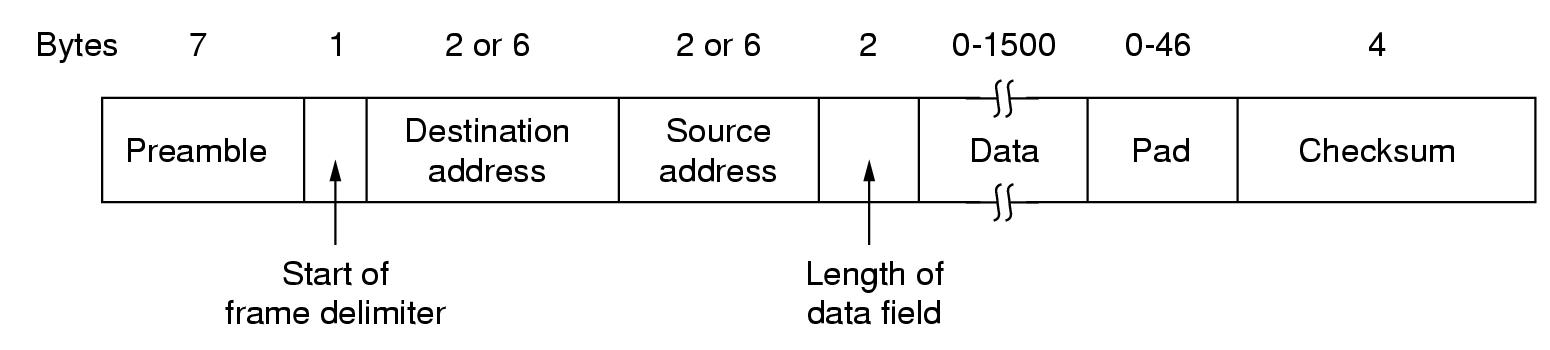
\includegraphics[width=.90\linewidth]{img/4-21.jpg} \\
		{\scriptsize Format de trame IEEE 802.3 (presque Ethernet) - Image de
		[Tanenbaum]}
	\end{center}
\end{itemize}
\end{frame}

\begin{frame}[fragile]
  \frametitle{Rappels réseaux - Ethernet}
{\large\bf Format de la trame Ethernet}
\begin{itemize}
	\item Préambule
	\begin{itemize}
		\item 8 fois 10101010b pour Ethernet
		\item 7 fois 10101010b pour 802.3, suivi du « Start of Frame » 10101011b
		\item Le codage Manchester de ces 8 \textit{bytes} produit un signal
		rectangulaire (10MHz pendant 6,4µs) permettant la synchronisation de l'horloge
	\end{itemize}
	\item Format des adresses
	\begin{itemize}
		\item Les champs adresses font 6 bytes
		\item Appelée « adresse MAC »; 3 premiers bytes pour le fabricant, 3 derniers pour la carte
		\item Différenciation
		\begin{itemize}
			\item Premier bit 0 pour adresse ordinaire
			\item Premier bit 1 pour adresse de groupe (diffusion \textit{multicast})
			\item Si tous les bits sont à 1 \textit{broadcast}
		\end{itemize}
	\end{itemize}
\end{itemize}
\end{frame}

\begin{frame}[fragile]
  \frametitle{Rappels réseaux - Ethernet}
{\large\bf Format de la trame Ethernet (suite)}
\begin{itemize}
	\item Type de la trame (Ethernet) ou longueur (802.3)
	\begin{itemize}
		\item Par exemple; 0x800 pour dire que la trame contient paquet IPv4
		\item Si la valeur est inférieure à 0x600, elle représente la longueur sinon, c'est le type
	\end{itemize}
	\item Données
	\begin{itemize}
		\item Maximum 1500 bytes
		\item Minimum 46 bytes (pour que la trame fasse minimum 64 bytes)
	\end{itemize}
\end{itemize}
\end{frame}

\begin{frame}[fragile]
  \frametitle{Rappels réseaux - Ethernet}
{\large\bf Format de la trame Ethernet (suite)}
\begin{itemize}
	\item Détection de collisions
	\begin{itemize}
		\item Le signal de brouillage peut mettre $2\tau$ pour revenir à l'émetteur 
		\item Dans LAN 10Mbit/s, $2\tau$ est proche de $50\mu s$  la trame
		doit donc avoir une longueur de 500 bits. On arrondi à 512 bits = 64
		bytes
	\end{itemize}
\end{itemize}
\begin{center}
	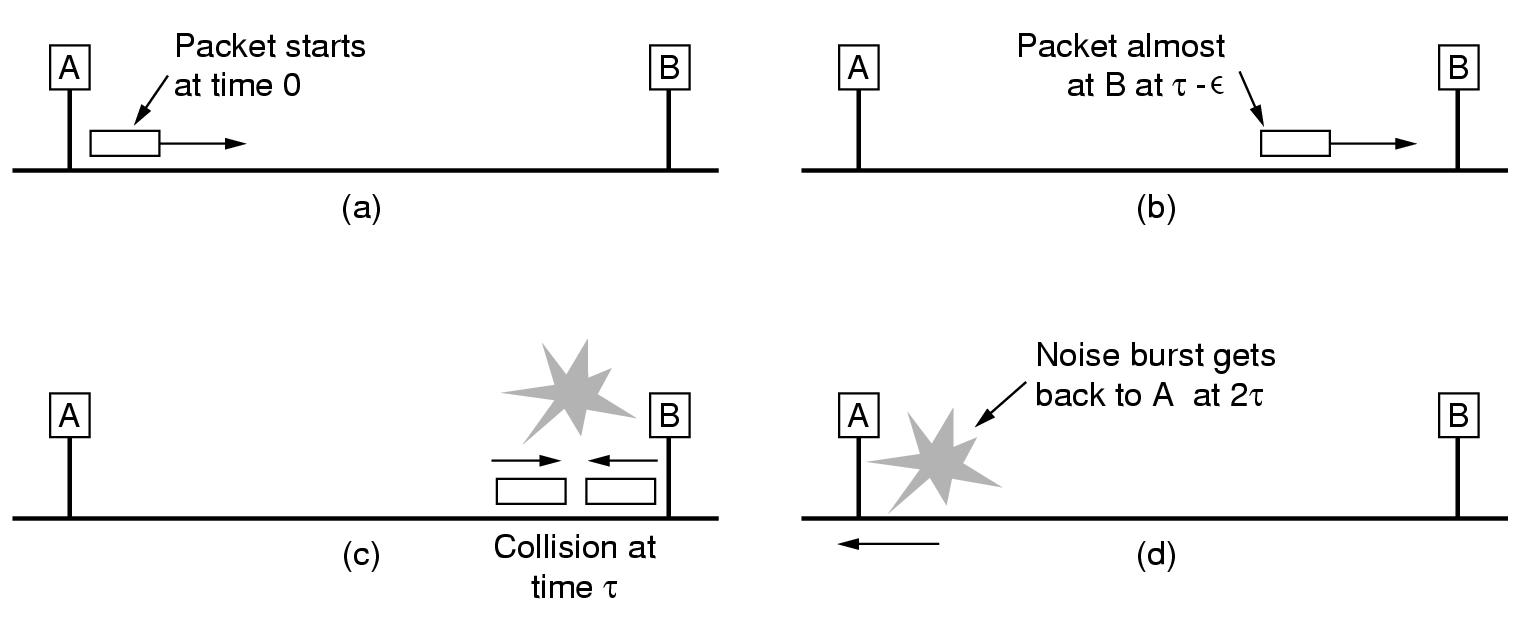
\includegraphics[width=.80\linewidth]{img/4-22.jpg} \\
	{\scriptsize Détection de colision - Image de [Tanenbaum]}
\end{center}
\end{frame}

\begin{frame}[fragile]
  \frametitle{Rappels réseaux - Ethernet}
{\large\bf Format de la trame Ethernet (suite)}
\begin{itemize}
	\item Total de contrôle (\textit{checksum})
	\begin{itemize}
		\item Si erreur, la trame est supprimée
		\item Valeur CRC de 32 bits
	\end{itemize}
\end{itemize}
\end{frame}


\begin{frame}[fragile]
  \frametitle{Rappels réseaux - Ethernet}
{\large\bf Exercice}
Observer le format d'une trame éthernet 
\begin{itemize}
	\item Utilisation de Wireshark
	\item Faire passer une trame et repérer les \textit{MAC address}
	\item Constater / vérifier que le mode promicuous ne fonctionne pas avec un switch
	\item Liens / références / aide
	\begin{itemize}
		\item Wireshark \url{http://www.wireshark.org}
		\item\url{http://wiki.wireshark.org/Ethernet}
	\end{itemize}
\end{itemize}
\end{frame}



\section{Ce qui différencie un LAN d'un WAN}

\begin{frame}[fragile]
  \frametitle{Ce qui différencie un LAN d'un WAN}
\begin{center}
	\Huge{\bf\color{blue}Ce qui différencie un LAN d'un WAN}
\end{center}
\begin{flushright}
  \item L'existant
  \item La couche physique
  \item La couche liaison de données
  \item La couche réseau
\end{flushright}
\end{frame}

\begin{frame}[fragile]
  \frametitle{Ce qui différencie un LAN d'un WAN}
\textbf{Couche physique}
\begin{itemize}
	\item Le support de transmission doit pouvoir laisser passer
	\textbf{beaucoup} plus de données que dans un LAN
	\begin{itemize}
		\item multiplexage
	\end{itemize}
	\item L'existant et les « nouveaux » types de support
	\begin{itemize}
		\item le réseau téléphonique commuté (xDSL)
		\item le câble
		\item la fibre optique (SONET)
	\end{itemize}
	\item Les différents intervenants
\end{itemize}
\textbf{Couche liaison de données}
	\begin{itemize}
		\item Protocoles de liaison de données
	\end{itemize}
\textbf{Couche réseau}
	\begin{itemize}
		\item Routage des paquets
	\end{itemize}
\end{frame}


\section{Multiplexage}

\begin{frame}[fragile]
  \frametitle{Multiplexage}
\begin{center}
	\Huge{\bf\color{blue}Multiplexage}
\end{center}
\begin{flushright}
	\item Multiplexage fréquentiel
	\item Multiplexage par répartition orthogonale de la la fréquence
	\item Multiplexage temporel
	\item Multiplexage par répartition de codes
	\item Multiplexage en longueur d'ondes
\end{flushright}
\end{frame}


\begin{frame}[fragile]
  \frametitle{Multiplexage}
{\bf\large  Multiplexage}\\
Consiste à partager une même ligne entre plusieurs signaux
\par Il est inenvisageable de «tirer» une ligne par signal
\end{frame}


\section{Multiplexage fréquentiel (FDM)}

\begin{frame}[fragile]
  \frametitle{Multiplexage fréquentiel (FDM)}
{\bf\large Multiplexage fréquentiel 
(\textit{FDM Frequency Division Multiplexing})}\\
Division du spectre en bandes de fréquences
\begin{itemize}
	\item Basé sur la transmission «passe bande»
	\begin{itemize}
		\item Un signal qui occupe de 0 à B Hz peut être décalé pour occuper une
		fréquence de S à S+B Hz
	\end{itemize}
	\item Division du spectre en bandes de fréquences, chaque utilisateur a la
	possession exclusive d'une bande
\end{itemize}
\vspace{1cm}
Exemples
\begin{itemize}
	\item la radiodiffusion AM
	\item réseaux téléphoniques, cellulaires, sans fil et satellitaires
\end{itemize}
\end{frame}

\begin{frame}[fragile]
  \frametitle{Multiplexage fréquentiel (FDM)}
\begin{center}
	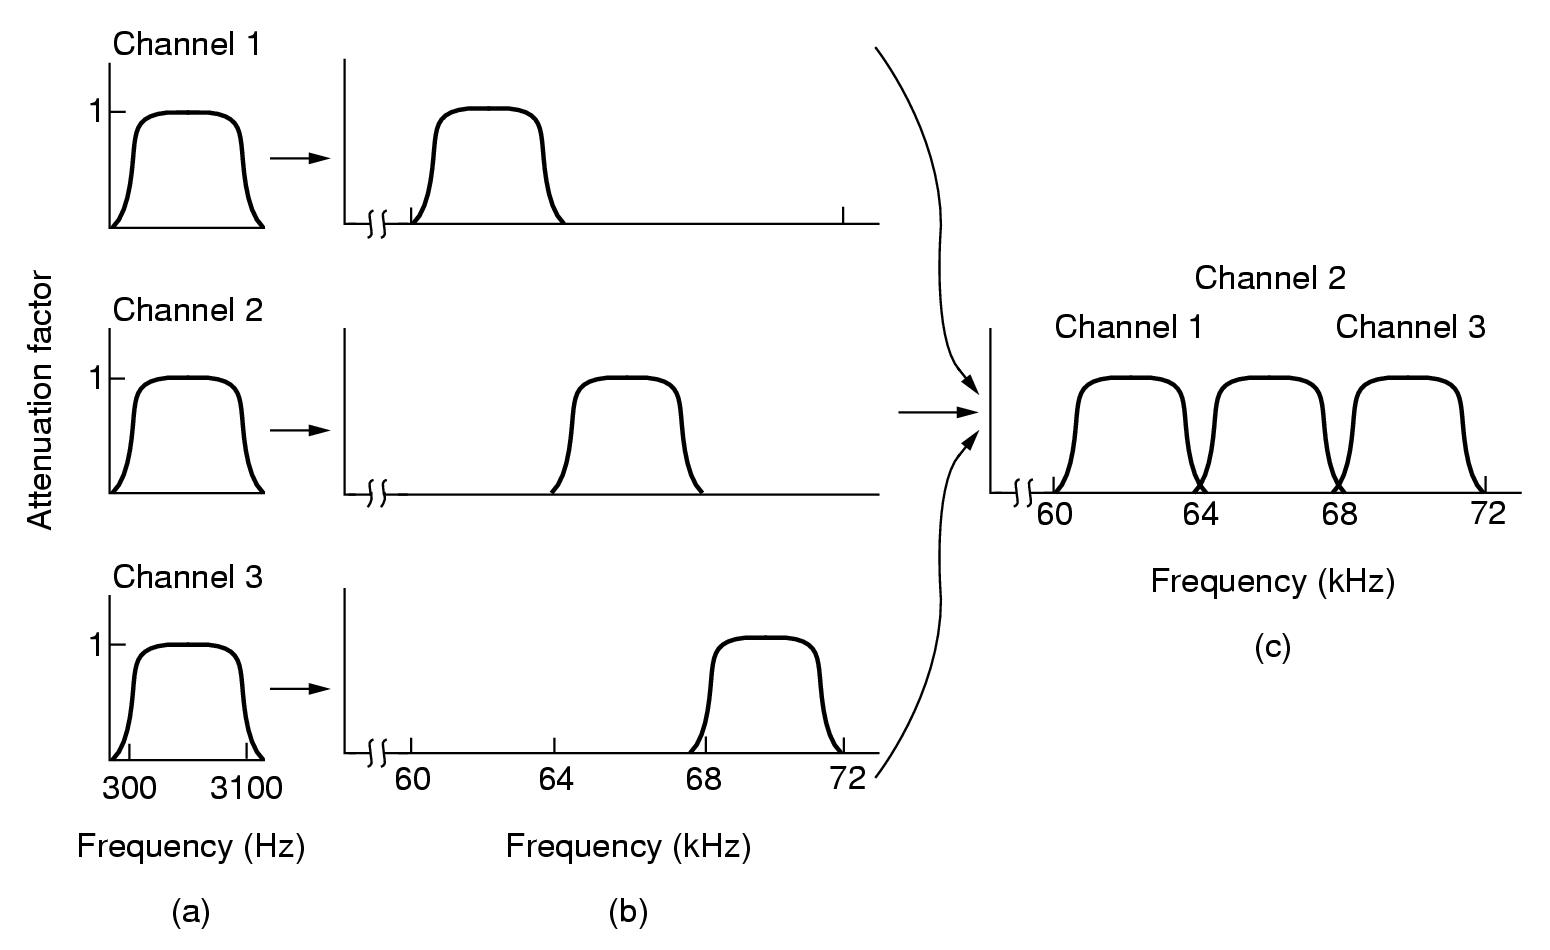
\includegraphics[width=.7\linewidth]{img/2-24.jpg}\\
	{\scriptsize FDM - Image de [Tanenbaum]}
\end{center}
\end{frame}

\begin{frame}[fragile]
	\frametitle{Transmission passe-bande}
{\large\bf Transmission passe-bande}
\par
En transmission passe-bande, la \textbf{modulation numérique} se fait en modifiant
\begin{itemize}
	\item l'amplitude (\textit{AFK Amplitude Shift Keying})
	\item la fréquence (\textit{FSK Frequence Shift Keying}) ou
	\item la phase (\textit{PSK Phase Shift Keying})
\end{itemize}
\end{frame}

\begin{frame}[fragile]
	\frametitle{Transmission passe-bande}
{\large\bf Transmission passe-bande}
\begin{center}
	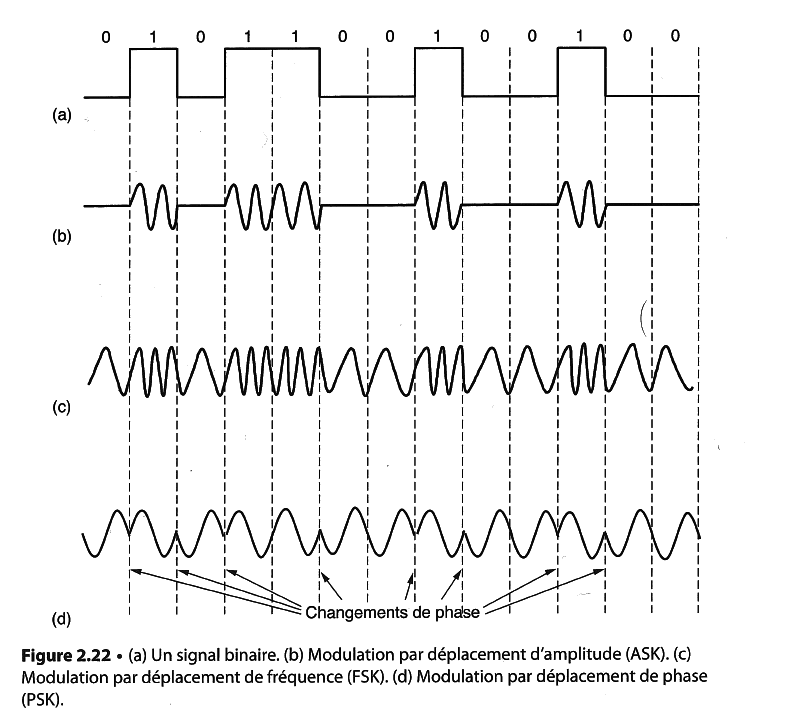
\includegraphics[width=.64\linewidth]{img/2-22.png} \\
	{\scriptsize From [Tanenbaum]}
\end{center}
\end{frame}

\begin{frame}[fragile]
	\frametitle{Transmission passe-bande}
{\large\bf \textit{BPSK Binary Phase Shift Keying}}
\begin{itemize}
	\item La porteuse est décalée de 0 ou $\pi$, soit \textbf{deux symboles}
	($\frac{2\pi}{2}$)
\end{itemize}
\vspace{1cm}
{\large\bf \textit{QPSK Quadrature Phase Shift Keying}}
\begin{itemize}
	\item On ne découpe plus en 2 mais en 4, soit 
	$\frac{\pi}{4}$, $\frac{3\pi}{4}$, $\frac{5\pi}{4}$ et $\frac{7\pi}{4}$
	\item Permet de représenter 4 symboles, soit 2 bits par symbole
\end{itemize}
\end{frame}

\begin{frame}[fragile]
	\frametitle{Transmission passe-bande}
{\large\bf \textit{QAM Quadrature Amplitude Modulation}}
\begin{itemize}
	\item Combinaison de PSK et AFK
	\item Permet de plusieurs symboles, on parle de \textbf{constellations}
\end{itemize}
\begin{center}
	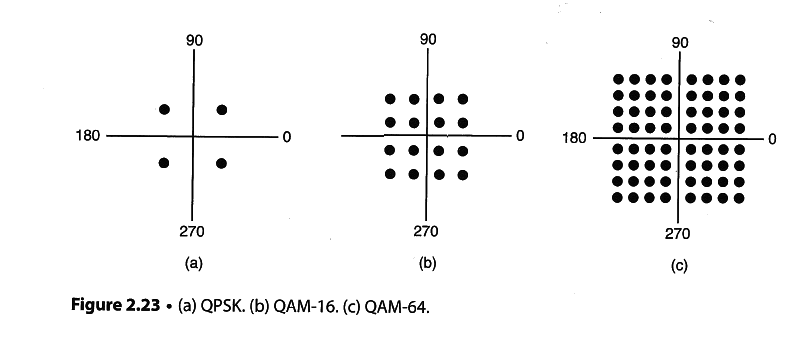
\includegraphics[width=.6\linewidth]{img/2-23.png}
\end{center}
\end{frame}

\begin{frame}[fragile]
	\frametitle{Transmission passe-bande}
{\large\bf \textit{QAM Quadrature Amplitude Modulation (suite)}}
\begin{itemize}
	\item QAM16, QAM64, ...
	\item Association des bits aux symboles de manière à minimiser 
	les erreurs dues au bruit, \textbf{code de Gray}
\end{itemize}
\begin{center}
	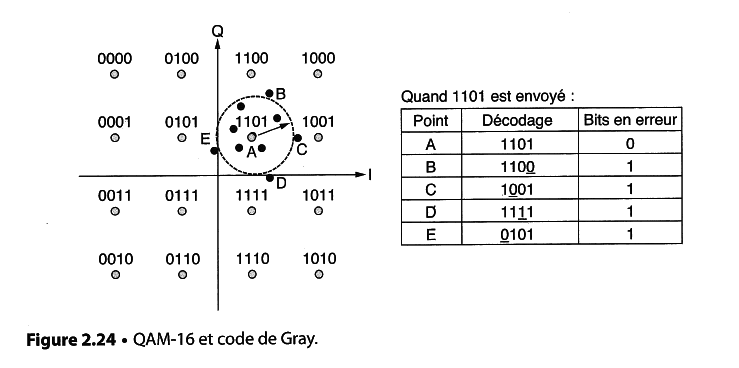
\includegraphics[width=.8\linewidth]{img/2-24.png}
\end{center}
\end{frame}

\section{Multiplexage par répartition orthogonal de la fréquence (OFDM)}

\begin{frame}[fragile]
  \frametitle{Multiplexage par répartition orthogonale de la fréquence (OFDM)}
{\large\bf Multiplexage par répartition orthogonale de la fréquence \\
(\textit{OFDM Orthogonal Frequency Division Multiplexing})}\\
Division du spectre en plusieurs sous-porteuses
\begin{itemize}
	\item Basé sur QAM (\textit{Quadrature Amplitude Modulation}), technique de
	modulation par variation de phase et de fréquence
	\item Les signaux de chaque sous porteuse se chevauchent mais s'annulent au
	centre car leurs fréquences sont orthogonales
\end{itemize}
\vspace{.6cm}
Exemples 
\begin{itemize}
	\item Très haut débit
	\item CPL (Courant porteur)
	\item 4G
	\item ADSL, VDSL
	\item câble
\end{itemize}
\end{frame}

\begin{frame}[fragile]
  \frametitle{Multiplexage par répartition orthogonale de la fréquence (OFDM)}
\begin{center}
	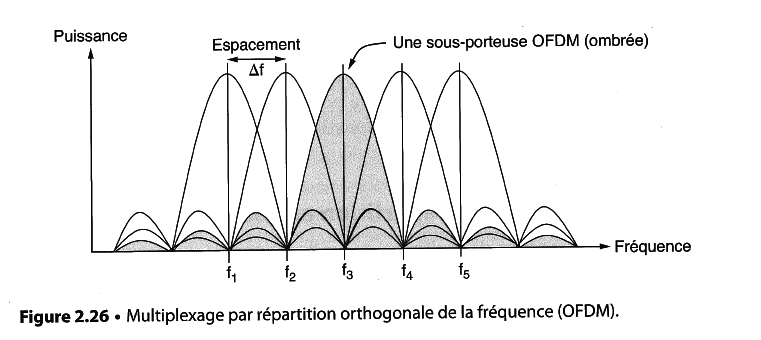
\includegraphics[width=.8\linewidth]{img/2-26.png}\\
	{\scriptsize OFDM - Image de [Tanenbaum]}
\end{center}
\end{frame}


\section{Multiplexage temporel (TDM)}

\begin{frame}[fragile]
  \frametitle{Multiplexage temporel (TDM)}
{\bf\large Multipdexage temporel \\
(\textit{TDM Time Division Multiplexing})}\\
Émission tour à tour
\begin{itemize}
	\item Chaque utilisateur émet à son tour sur l'intégralité de la bande passante
\end{itemize}
\vspace{1cm}
Exemple
\begin{itemize}
	\item Réseaux téléphoniques et cellulaires
\end{itemize}
\end{frame}

\section{Multiplexage temporel TDM}

\begin{frame}[fragile]
  \frametitle{Multiplexage temporel TDM}
\begin{center}
	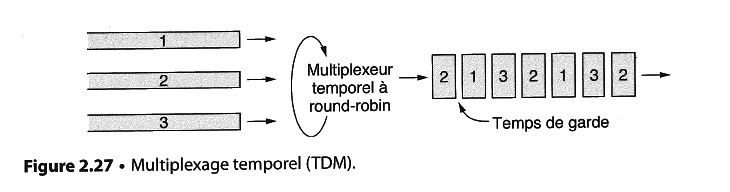
\includegraphics[width=.8\linewidth]{img/2-27.png}\\
	{\scriptsize TDM - Image [Tanenbaum]}
\end{center}
\end{frame}



\section{Multiplexage par répartition en codes CDMA}

\begin{frame}[fragile]
  \frametitle{Multiplexage par répartition en codes (CDMA)}
{\large\bf Multiplexage par répartition de codes \\
(\textit{CDMA Code Division Multiple Access})}\\
Plusieurs utilisateurs utilisent la même bande de fréquence
\begin{itemize}
	\item Tout le monde émet sur la même fréquence
	\item Plusieurs émissions se distinguent car elles sont codées différement
\end{itemize}
\end{frame}

\begin{frame}[fragile]
  \frametitle{Multiplexage par répartition en codes (CDMA)}
\textbf{Fonctionnement}
\begin{itemize}
	\item Chaque temps bit est divisé en \textit{m} courts intervalles
	(\textbf{chips})
	\item \textit{m} vaut généralement 64 ou 128 (dans l'exemple, $m=8$)
	\item Chaque station reçoit une \textbf{séquence de chips} unique et telle
	que deux séquences $S$ et $T$ quelconque ont un produit nul $S\bullet T$
	$$S\bullet T = \frac{1}{m}\sum^m_{i=1}S_iT_i$$
	\begin{itemize}
		\item Exemple (-1, -1, -1, +1, +1,-1, +1, +1)
	\end{itemize}
	\item Pour émettre 1, émission de la séquence de chips
	\item Pour émettre 0, émission de la \textbf{négation} de la séquence
\end{itemize}
\end{frame}

\begin{frame}[fragile]
  \frametitle{Multiplexage par répartition en codes (CDMA)}
\begin{center}
	\item 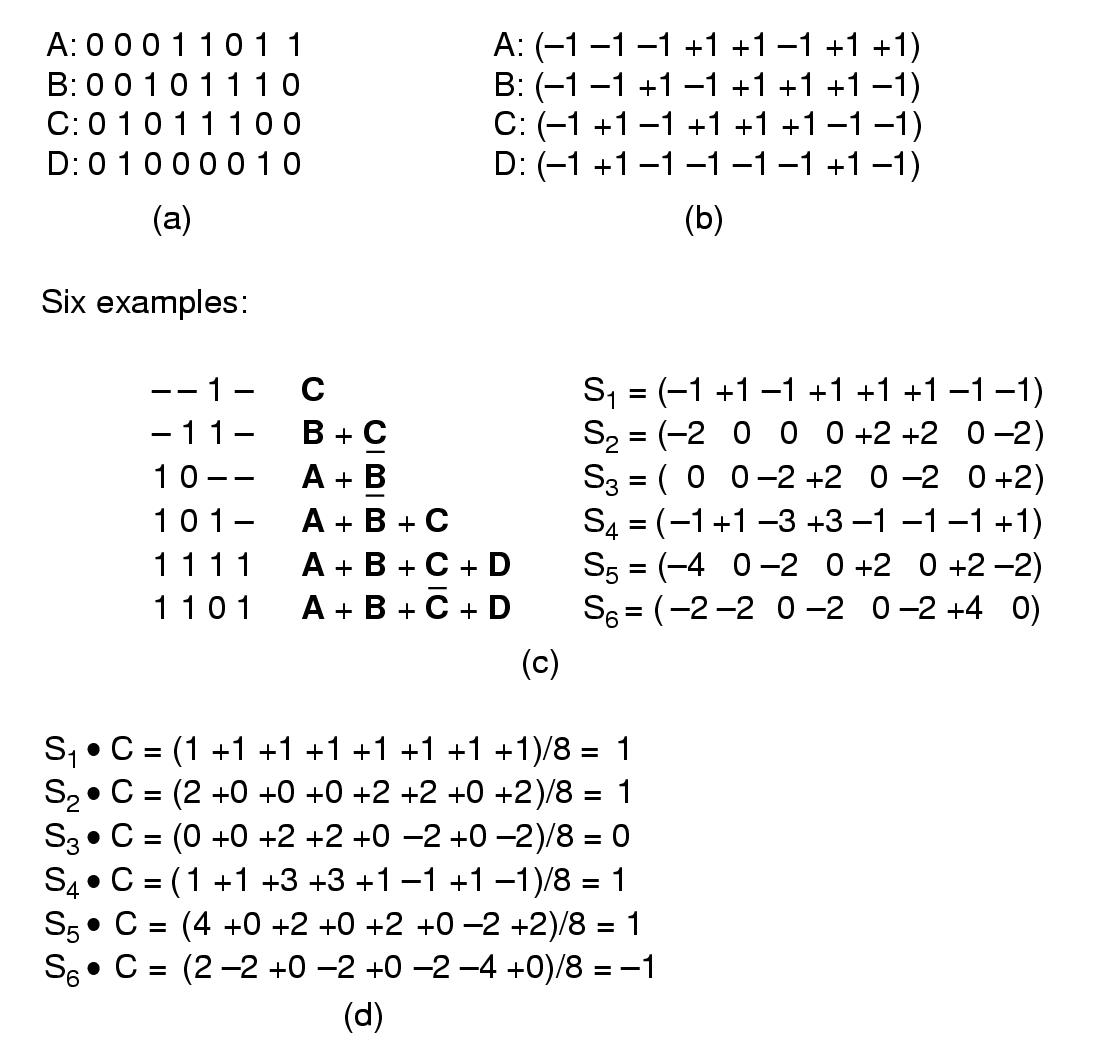
\includegraphics[width=.56\linewidth]{img/4-16.jpg}\\
	{\scriptsize Exemple CDMA - Image [Tanenbaum]}
\end{center}
\end{frame}

\section{Multiplexage en longueur d'ondes (WDM)}

\begin{frame}[fragile]
  \frametitle{Multiplexage en longueur d'ondes (WDM)}
{\large\bf Multiplexage en longueur d'ondes  \\
(\textit{WDM Wavelength Division Multiplexing})}
\begin{itemize}
	\item Sorte de multiplexage fréquentiel à très hautes fréquences
	\item Destiné à la fibre optique (grande bande passante)
\end{itemize}
\vspace{.5cm}
\textbf{Fonctionnement}
\begin{itemize}
	\item Chaque fibre arrive sur un prisme
	\item Les flux, d'énergie et de longueur d'onde spécifique, sont combinés
	\item À la sortie, le faisceau est séparé
\end{itemize}
\end{frame}

\begin{frame}[fragile]
  \frametitle{Multiplexage en longueur d'ondes (WDM)}
\begin{center}
	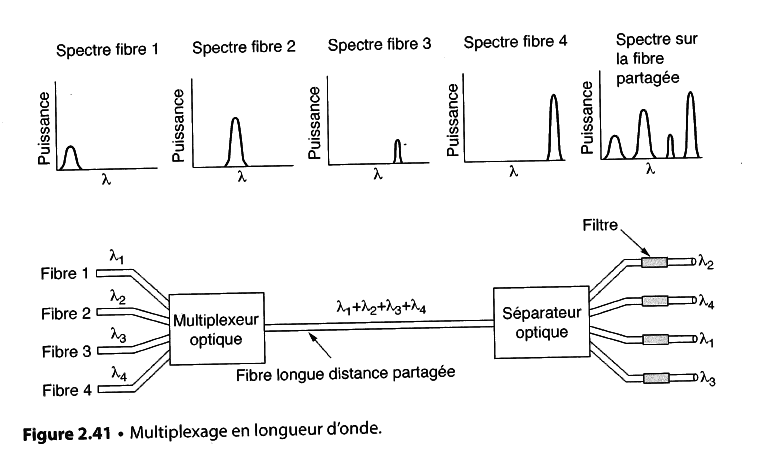
\includegraphics[width=.8\linewidth]{img/2-41.png}\\
	{\scriptsize WDM - Image [Tanenbaum]}
\end{center}
\end{frame}



\section{RTC - Le réseau téléphonique commuté}

\begin{frame}[fragile]
	\frametitle{Le réseau téléphonique commuté}
\begin{center}
	\Huge{\bf\color{blue}Le réseau téléphonique commuté \\ 
	\LARGE\it PSTN Public Switched telephone Network}
\end{center}
\begin{flushright}
  \item Présentation
  \item La boucle locale
  \item Artères interurbaines (\textit{Backbone})
  \item Les centres de commutations
\end{flushright}
\end{frame}


\begin{frame}[fragile]
  \frametitle{Le réseau téléphonique commuté}
{\large\bf Réseau Téléphonique Commuté (RTC) \\
(\textit{Public Switched Telephone Network (PSTN)}}\\
\textit{«Ce qui coûte le plus cher, c'est de creuser les tranchées»}
\begin{itemize}
	\item Impose de s'appuyer sur RTC
	\item Avec l'arrivée de la fibre, reste encore le problème du «dernier km»
	\item RTC est conçu pour laisser passer la voix ... pas les datas
\end{itemize}
\vspace{1cm}
\textit{Un câble croisé permet le 1Gbit/s, l'ADSL permet 1Mbit/s ... et RTC
(permettait) 56kbit/s}
\end{frame}

\begin{frame}[fragile]
  \frametitle{Le réseau téléphonique commuté}
{\large\bf Structure avec interconnexion totale}
\begin{itemize}
	\item Chaque téléphone est relié à son destinataire.
	\item C'est l'époque de \textit{Graham Bell} (et d'\textit{Elisha Gray}) (1876)
\end{itemize}
\begin{center}
	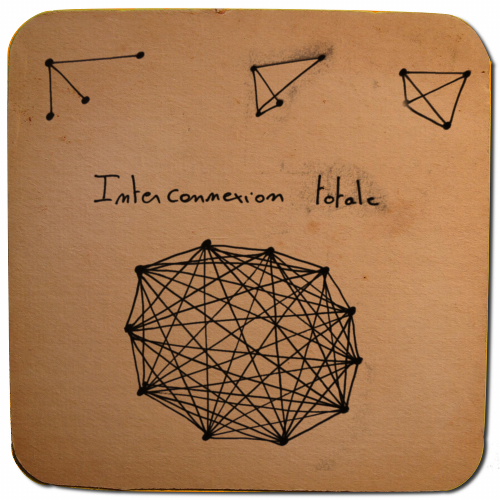
\includegraphics[width=.53\linewidth]{img/sousbock-rtc-interconnexiontotale.png}
	\par{\scriptsize Image de [Tanenbaum]} 
\end{center}
\end{frame}

\begin{frame}[fragile]
  \frametitle{Le réseau téléphonique commuté}
{\large\bf Réseau avec commutateur central}
\begin{itemize}
	\item Chaque téléphone est relié au commutateur central
	\item C'est l'époque de la \textit{Bell Telephone Company} créée par Graham Bell (1878)
\end{itemize}
\begin{center}
	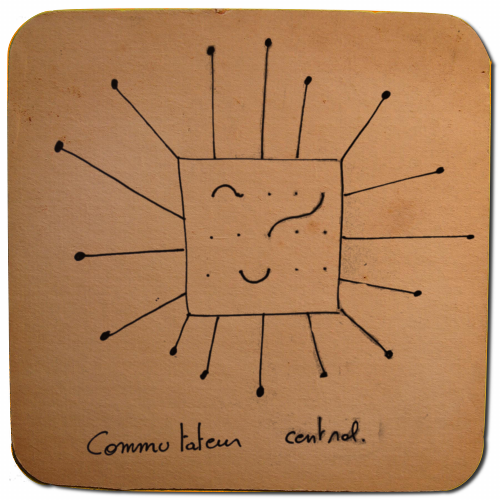
\includegraphics[width=.5\linewidth]{img/sousbock-rtc-commutateurcentral.png}
\end{center}
\end{frame}

\begin{frame}[fragile]
  \frametitle{Le réseau téléphonique commuté}
{\large\bf Réseau hiérarchique à plusieurs niveaux}
\begin{itemize}
	\item Nécessité de connecter plusieurs villes ... apparaissent les centrales
	de second niveau
	\item Système BELL
\end{itemize}
\begin{center}
	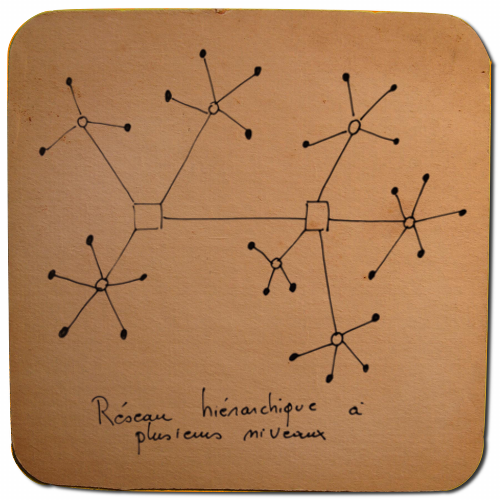
\includegraphics[width=.5\linewidth]{img/sousbock-rtc-hierarchique.png}
\end{center}
\end{frame}

\begin{frame}[fragile]
  \frametitle{Le réseau téléphonique commuté}
{\large\bf Réseau hiérarchique à plusieurs niveaux (avec redondance)}
\begin{itemize}
	\item Permet plusieurs chemins ... \textbf{routage}
\end{itemize}
\begin{center}
	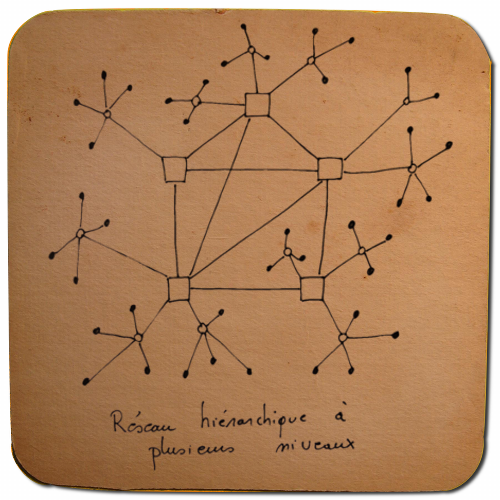
\includegraphics[width=.54\linewidth]{img/sousbock-rtc-hierarchiqueroutage.png}
\end{center}
\end{frame}

\begin{frame}[fragile]
  \frametitle{Le réseau téléphonique commuté}
{\large\bf Les éléments du système téléphonique}
\begin{itemize}
	\item La \textbf{boucle locale (\textit{local loop})}
	\begin{itemize}
		\item longue de 1 à 10km
		\item \textit{relie l'utilisateur au ...}
	\end{itemize}
	\item \textbf{commutateur local (\textit{local central office}) CL}
	\begin{itemize}
		\item paire de fils de cuivre torsadés
		\item si les abonnés sont dans le même central, le CL établit la connexion
		\item \textit{sinon ...}
	\end{itemize}
	\item \textbf{commutateur à autonomie d'acheminement (\textit{Toll office}) CAA}
	\begin{itemize}
		\item deuxième niveau de commutation
		\item forme une ZAA (Zone à autonomie d'acheminement)
		\item reliés aux CL par une \textbf{artère principale (\textit{trunk})}
	\end{itemize}
	\item \textbf{commutateur de transit secondaire (CTS)}
	\begin{itemize}
		\item troisième niveau de commutation
	\end{itemize}
	\item \textbf{commutateur de transit primaire (CTP)}
	\begin{itemize}
		\item quatrième niveau de commutation
	\end{itemize}
\end{itemize}
\end{frame}

\begin{frame}[fragile]
  \frametitle{Le réseau téléphonique commuté}
\begin{center}
	IMG
\end{center}
\end{frame}

\begin{frame}[fragile]
  \frametitle{Le réseau téléphonique commuté}
{\large\bf Évolution historique}
\begin{itemize}
	\item 1984 Fin du monopole de BELL System par le bais du 
	\textit{Modified Final Judgment (\textbf{MFJ})}
	\begin{itemize}
		\item découpage des USA en 164 \textbf{zones d'accès local 
		(LATA \textit{Local Access and Transport Area}}) controlées par un
		opérateur local (\textit{LEC Local Exchange Carrier}
		\item trafic inter-LATA géré par un autre opérateur,
		\textbf{IXC \textit{IntereXchange Carrier}} (AT\&T, Verizon et Sprint)
		\item Pour traiter un appel provenant d'une LATA, un IXC a besoin d'un
		centre de commutation dans la zone appelé \textbf{point de présence (POP
		\textit{Point Of Presence})}
	\end{itemize}
	\item 1996 Fin de la distinction LEC / IXC ... tout le monde peut occuper
	les différents types de marché; câble, téléphonie locale, téléphonie longue
	distance et téléphonie mobile
	\begin{itemize}
	 	\item Corrolaire: portabilité des numéros d'abonné local
	\end{itemize}
	\item 2003 Portabilité des numéros de mobiles
\end{itemize}
\end{frame}

\section{RTC - La boucle locale}

\begin{frame}[fragile]
	\frametitle{La boucle locale}
\begin{center}
	{\Huge\bf\color{blue} La boucle locale}
\end{center}
\end{frame}

\begin{frame}[fragile]
  \frametitle{La boucle locale}
{\large\bf La \textbf{boucle locale} ou \textit{«le dernier kilomètre»}}
\begin{itemize}
	\item Paire de fils de cuivre de l'abonné au \textit{toll office}
	(Commutateur Local ou Commutateur à Autonomie d'Acheminement) 
	\item Nécessite une transformation numérique $\rightarrow$ analogique par le
	biais d'un \textbf{modem}
\end{itemize}
\end{frame}



\section{RTC - Ateliers de recherche 1}

\begin{frame}[fragile]
	\frametitle{RTC - La boucle locale - Ateliers de recherche 1}
{\large\bf Ateliers de recherche 1} 
\begin{itemize}
	\item Sur base des pages 156 à 163 de [Tanenbaum], expliquer, comprendre, … 
	\begin{itemize}
		\item le modem téléphonique
		\item le modem xDSL
		\item la fibre FTTx (\textit{Fibre to the home})
	\end{itemize}
	\item Rédiger un document en groupe pour un des 3 points et le présenter aux autres
	groupes
\end{itemize}
\end{frame}



\section{RTC - Artères interurbaines (backbones)}

\begin{frame}[fragile]
	\frametitle{RTC - Artères interurbaines (backbones)}
\begin{center}
	{\Huge\bf\color{blue} RTC - Artères interurbaines (backbones)}
\end{center}
\end{frame}


\begin{frame}[fragile]
  \frametitle{RTC - Artères interurbaines (\textit{backbones})}
{\large\bf Préalables}
\begin{itemize}
	\item Plusieurs signaux sont \textbf{multiplexés}
	\begin{itemize}
		\item TDM (\textit{time division multiplexing})
		\item FDM (\textit{frequency division multiplexing})
	\end{itemize}
	\item Les boucles locales produisent un signal analogique 
	qui doit être numérisé par un \textbf{codec}
\end{itemize}
\end{frame}

\begin{frame}[fragile]
	\frametitle{RTC - Artères interurbaines (\textit{backbones})}
{\large\bf PCM Pulse Code Modulation} \\
PCM est une technique d'échantillonage
\begin{itemize}
	\item Le codec prélève 8000 échantillons par seconde
	(125 $\mu s$/échantillon)
	\item 8000 échantillons, 2 fois la fréquence de 4000Hz
	\item Chaque échantillon est transformé en nombre de 8 bits
	\item Débit binaire standard 64kbit/s ($2\times4000(Hz)\times8(bits)$)
\end{itemize}
\end{frame}

\begin{frame}[fragile]
	\frametitle{RTC - Artères interurbaines (\textit{backbones})}
{\large\bf Multiplexage temporel}
\begin{itemize}
	\item Envoi de plusieurs signaux en envoyant 1 échantillon de chaque appel toutes les 125$\mu s$
	\item Deux techniques cohabitent
	\begin{itemize}
		\item Technique \textbf{T1}, norme G.733 (États-unis et Japon)
		\item Technique \textbf{E1}, norme G.732 (Europe)
	\end{itemize}
\end{itemize}
\end{frame}

\begin{frame}[fragile]
  \frametitle{RTC - Artères interurbaines (\textit{backbones})}
{\large\bf Multiplexage temporel - Technique T1}
\begin{itemize}
	\item 24 voies téléphoniques multiplexée ensemble
	\item Toutes les 125$\mu s$, une trame est construite en prélevant 8 bits
	sur chaque voie, soit $24\times 8 = 192 bits$ plus 1 bit de contrôle
	\item Une ligne T1 fournit un débit (théorique) de 1,544Mbits/s ($8000\times
	193$) dont 8kbits/s pour la signalisation
	\item Le $193^e$ bit est le \textbf{bit de verrouillage de trame}
\end{itemize}
\end{frame}

\begin{frame}[fragile]
	\frametitle{RTC - Artères interurbaines (\textit{backbones})}
{\large\bf Multiplexage temporel - Technique T1 (suite)}
\begin{center}
	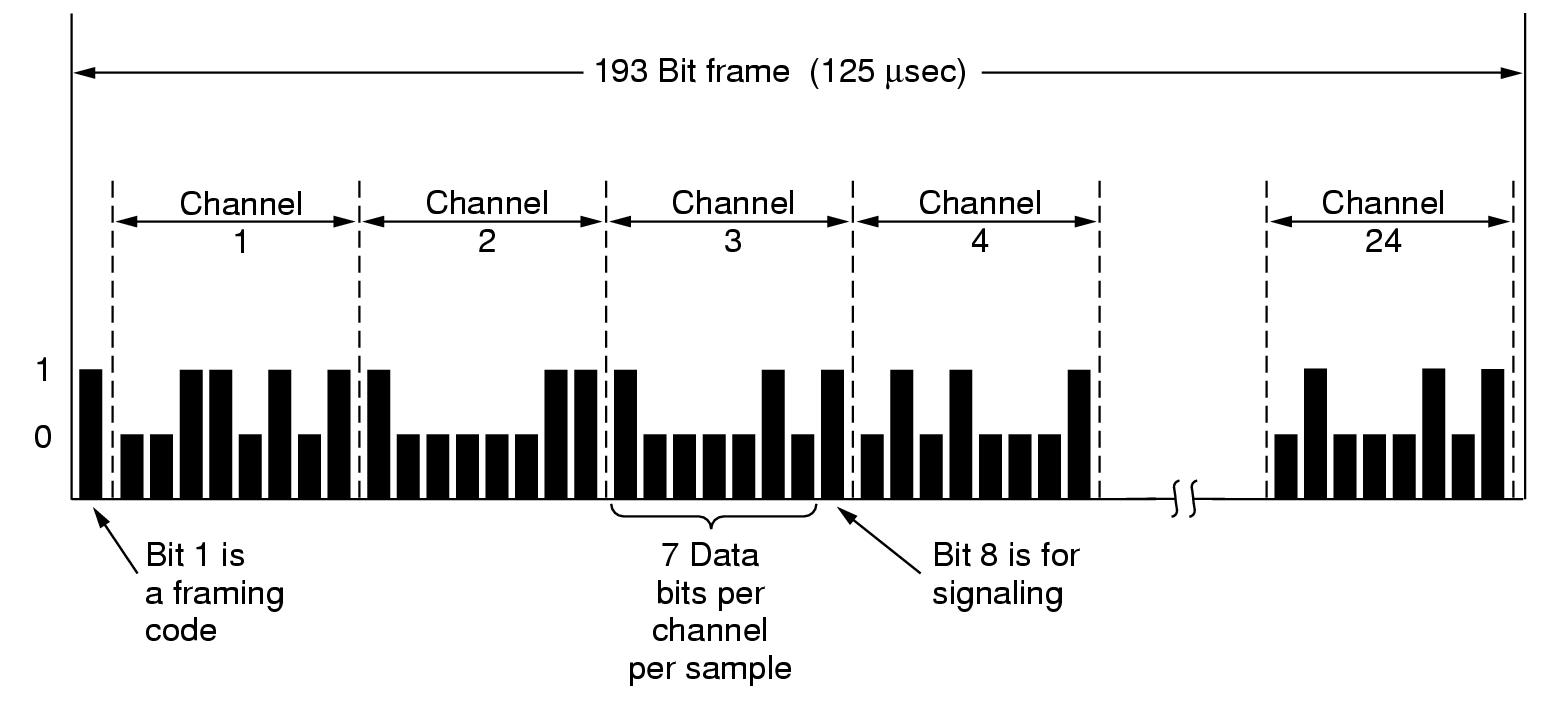
\includegraphics[width=.8\linewidth]{img/2-26-old.jpg}
	\par{\scriptsize Image de [Tanenbaum]} 
\end{center}
\end{frame}

\begin{frame}[fragile]
	\frametitle{RTC - Artères interurbaines (\textit{backbones})}
{\large\bf Multiplexage temporel - Technique E1}
\begin{itemize}
	\item 32 voies téléphoniques multiplexée ensemble
	\item $32\times 8 = 256 bits$
	\item les 8 bits sont utilisés pour les données mais les échantillons 0 et 16 
	sont utilisés pour la signalisation
	\item chaque échantillon est nommé «intervalle de temps» ou \textbf{slot}
	\item une ligne E1 fournit un débit (théorique) de 2,048Mbits/s ($8000\times
	256$) 
\end{itemize}
\end{frame}

\begin{frame}[fragile]
  \frametitle{RTC - Artères interurbaines (\textit{backbones})}
{\large\bf Multiplexage temporel - TDM}
\begin{itemize}
	\item Le multiplexage temporel permet de grouper plusieurs lignes T1 (États-Unis et Japon) 
	ou E1 (Europe)
	\item T1 T2 T3 T4
	\begin{itemize}
		\item T2 = 4 T1 (6.312 Mbits/s)
		\item T3 = 7 T2 (44.736 Mbits/s)
		\item T4 = 6 T3 (274.176Mbits/s)
	\end{itemize}
	\item E1 E2 E3 E4
	\begin{itemize}
		\item E2 = 4 E1 (8.848 Mbits/s)
		\item E3 = 4 E2 (34.304 Mbits/s)
		\item E4 =  4 E3 (139.264 Mbits/s)
	\end{itemize}
\end{itemize}
\end{frame}

\begin{frame}[fragile]
	\frametitle{RTC - Artères interurbaines (\textit{backbones})}
\begin{center}
	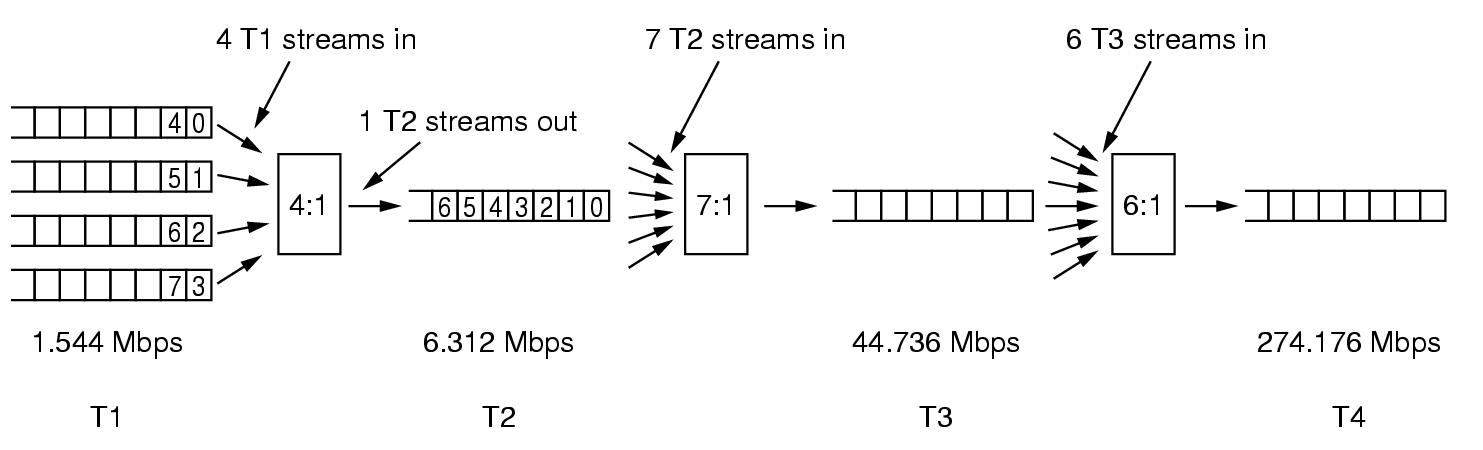
\includegraphics[width=.9\linewidth]{img/2-28-old.jpg}
	\par{\scriptsize Image de [Tanenbaum]} 
\end{center}
\end{frame}



\section{RTC - Ateliers de recherche 2}

\begin{frame}[fragile]
	\frametitle{RTC - Backones - Ateliers de recherche 2}
{\large\bf Ateliers de recherche 2} 
\begin{itemize}
	\item Sur base des pages 167 à 170 de [Tanenbaum], expliquer, comprendre, …
	\textbf{SONET (Synchronous Optical NETwork)}
\end{itemize}
\end{frame}



\section{RTC - Centres de commutation (central office)}

\begin{frame}[fragile]
  \frametitle{RTC - Centres de commutation (central office)}
{\Large\bf RTC - Centres de commutation (central office)}\\
{\large\bf Préalables}
\begin{itemize}
	\item Infrastructure extérieure
	\begin{itemize}
		\item boucle locale (\textit{local loop})
		\item artères principales (\textit{trunk / backbones})
	\end{itemize}
	\item Infrastructure intérieure
	\begin{itemize}
		\item centres de commutation
	\end{itemize}
\end{itemize}
\vspace{.5cm}
Techniques de commutation
\begin{itemize}
	\item commutation de circuits
	\item commutation de paquets
\end{itemize}
\end{frame}

\begin{frame}[fragile]
	  \frametitle{RTC - Centres de commutation (central office)}
{\large\bf Commutation de circuits}
\begin{itemize}
	\item Système téléphonique traditionnel
	\item Principe: recherche d'un chemin de bout en bout avant la transmission des données
	\item Nécessite un délai d'établissement de circuits
	\item Lorsque le chemin est réservé,
	\begin{itemize}
		\item transmission à la vitesse de propagation electromagnétique (5ms/1000km)
		\item pas de congestion
	\end{itemize}
	\item \textbf{Service garanti avec risque de gaspillage de la bande passante}
	\item Facturation à la durée et à la distance
\end{itemize}
\end{frame}

\begin{frame}[fragile]
  \frametitle{RTC - Centres de commutation (central office)}
{\large\bf Commutation de paquets}
\begin{itemize}
	\item Progression grâce à la \textit{voIP}
	\item Les paquets sont envoyés dès qu'ils sont disponibles, ils peuvent
	arriver dans le dérordre
	\item Transmission différée (\textit{store and forward})
	\item Risque de congestion et délai de mise en file
	\item Meilleure tolérance aux pannes (route alternative possible)
	\item \textbf{Service non garanti mais sans gaspillage de bande passante}
	\item Facturation au volume de données
\end{itemize}
\end{frame}

\begin{frame}[fragile]
  \frametitle{RTC - Centres de commutation (central office)}
\begin{center}
	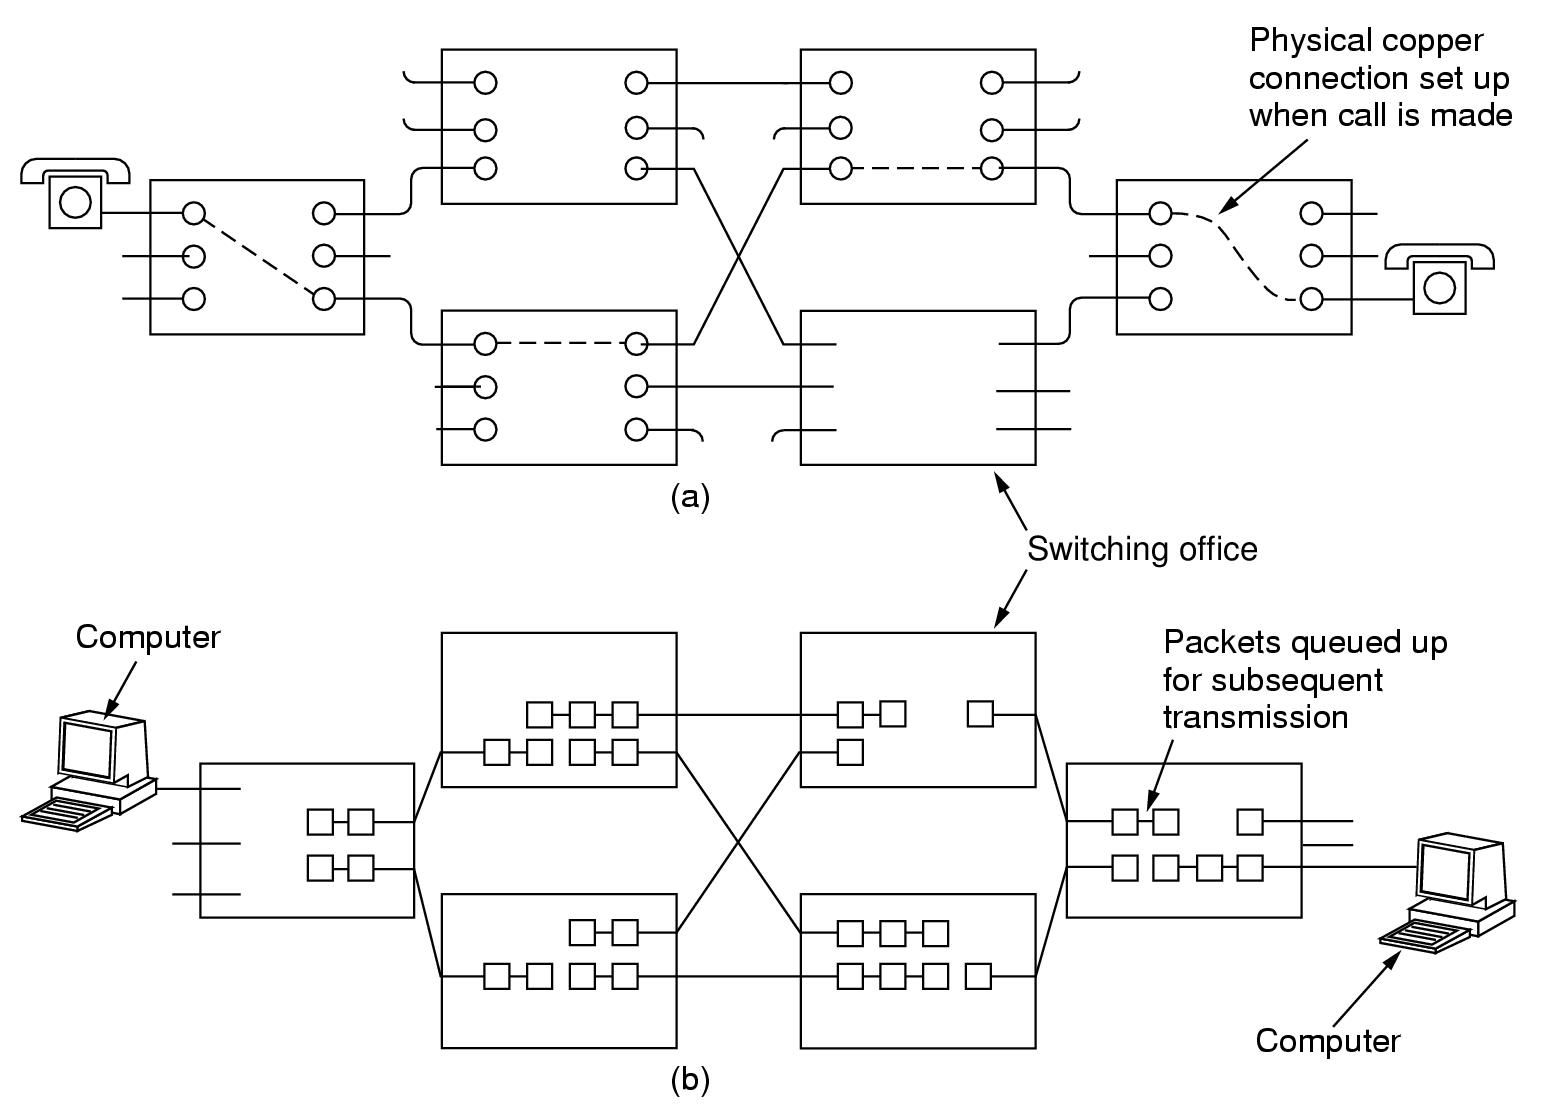
\includegraphics[width=.8\linewidth]{img/2-34-old.jpg}
	\par{\scriptsize (a) Commutation de circuit  (b) Commutation de paquets 
	\\ Image de [Tanenbaum]} 
\end{center}
\end{frame}



\section{RTC - Ateliers de recherche 3}

\begin{frame}[fragile]
	\frametitle{RTC Réseau de télévision câblé - Ateliers de recherche 3}
{\large\bf Ateliers de recherche 3} 
\begin{itemize}
	\item Sur base des pages 192 à 198 de [Tanenbaum], expliquer,
	comprendre,$\cdots$
	\begin{center}
		\textbf{\large le réseau de télévision câblée}
	\end{center}
	\item Rédiger un document commun présentant quelques points de comparaison
	entre \textbf{xDSL} sur le réseau téléphonique commuté et
	l'\textbf{internet par le câble}. 
\end{itemize}
\end{frame}


\section{Protocoles de la couche liaison de données}

\begin{frame}[fragile]
	\frametitle{Protocoles de la couche liaison de données}
\begin{center}
	\Huge{\bf\color{blue}Protocoles de la couche liaison de données}
\end{center}
\begin{flushright}
\end{flushright}
\end{frame}

\begin{frame}[fragile]
  \frametitle{ Protocoles de la couche de liaison}
\begin{itemize}
	\item Au niveau de la couche physique, ce sont des \textbf{bits} qui circulent sur un support
	\item Au niveau de la couche liaison de données, ce sont des \textbf{trames} qui circulent
	\item Une trame est un ensemble de bits qui encapsule un paquet (éventuellement découpé) de la couche réseau
\end{itemize}
\begin{center}
	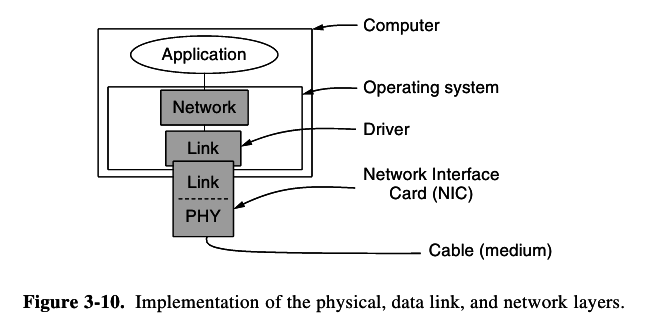
\includegraphics[width=.53\linewidth]{img/3-10.png}
	\par{\scriptsize Image de [Tanenbaum]} 
\end{center}
\end{frame}

\begin{frame}[fragile]
  \frametitle{Protocoles de la couche de liaison}
{\large\bf Protocole simplex utopique}
\begin{center}
	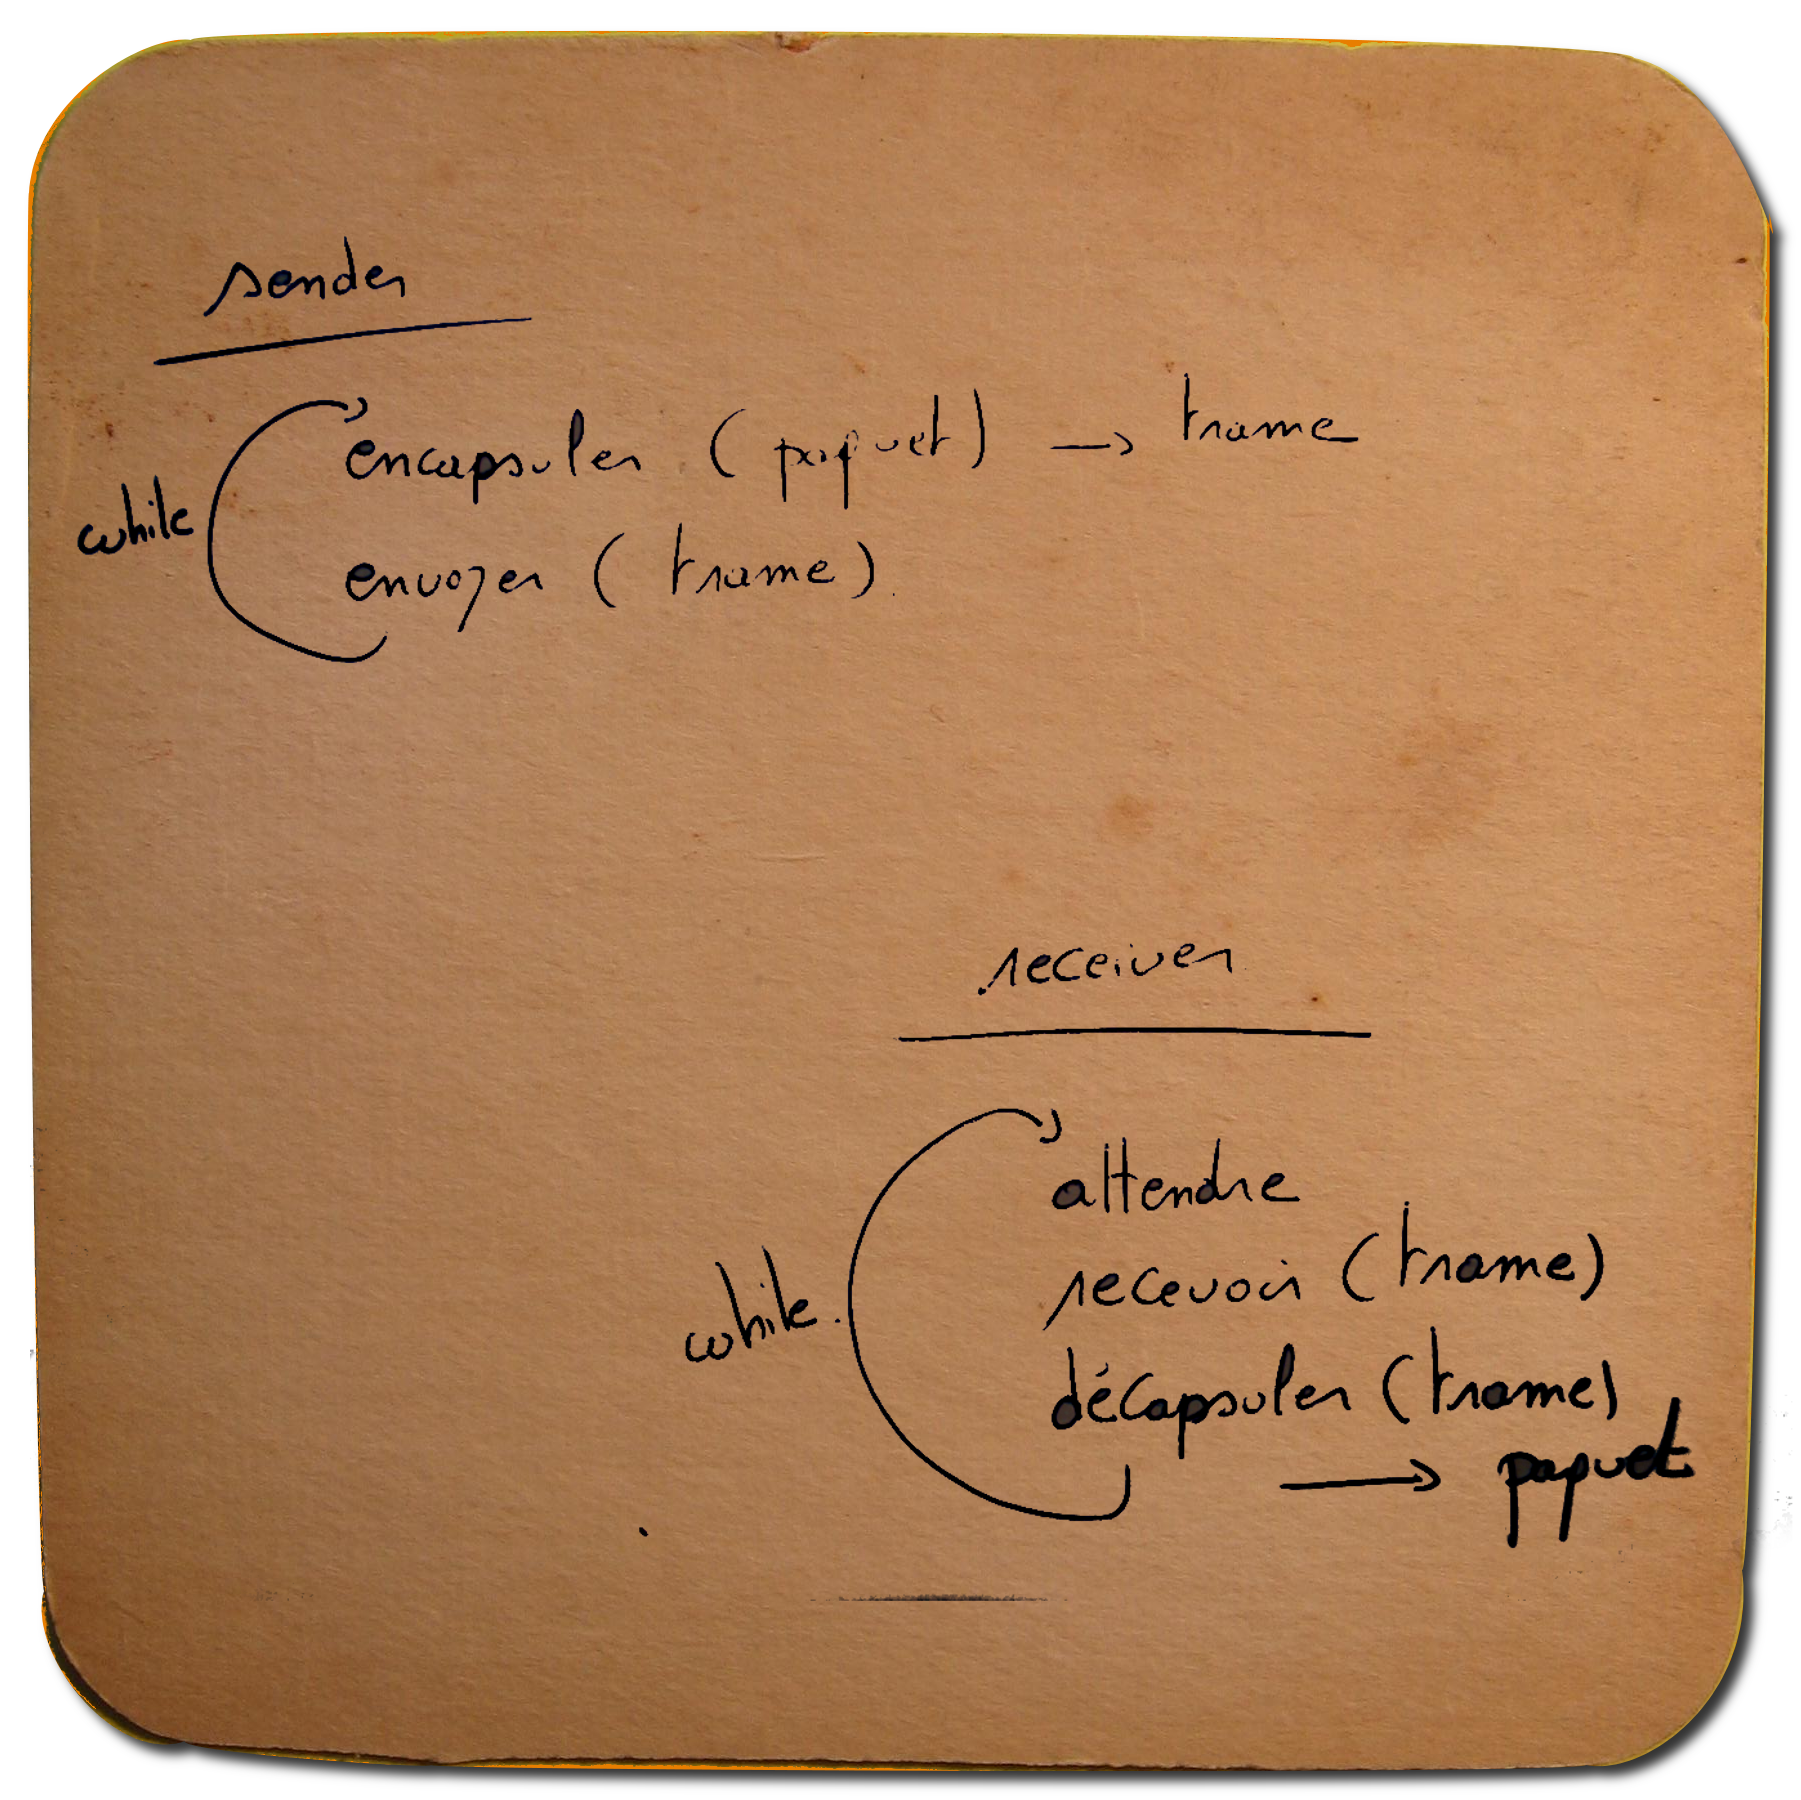
\includegraphics[width=.4\linewidth]{img/sousbock-protocole-1.png}
\end{center}
\begin{itemize}
	\item pas de contrôle de flux (risque d'inondation)
	\item pas de correction d'erreurs
	\item pas de gestion de perte ou de trames erronées
\end{itemize}
\end{frame}

\begin{frame}[fragile]
  \frametitle{ Protocoles de la couche de liaison}
\begin{itemize}
	\item Trivialement, les trames sont envoyées en continu mais
	\begin{itemize}
		\item le débit est limité
		\item le délai de propagation est non nul
		\item des erreurs de transmission peuvent survenir
	\end{itemize}
\end{itemize}
\begin{center}
	\bf Comment résoudre ces problèmes ?
\end{center}
\end{frame}

\begin{frame}[fragile]
	\frametitle{Protocoles de la couche de liaison}
{\large\bf Ateliers de recherche 4}
\begin{itemize}
	\item Sur base des pages 225 à 241 de [Tanenbaum], comprendre les protocoles
	3,4,5 et 6
	\item Écrire un programme (en Java, C ou Python) permettant d'illustrer le
	protocole 3. 
\end{itemize}
\end{frame}

%\begin{frame}[fragile]

%  \frametitle{Protocoles de la couche de liaison}
%\begin{itemize}
%\item Protocole simplex, stop and wait, sans bruit
%\item Protocole simplex, stop and wait, canal bruité
%\item Protocoles avec fenêtre d'anticipation
%\end{itemize}
%\end{frame}




\section{Crédits}

\begin{frame}[fragile]
  \frametitle{Crédits}
\begin{itemize}
	\item \textbf{GNU / linux} comme OS et sa suite d'outils
	\item \textbf{freeplane} - http://freeplane.sourceforge.net  \\ 
	\textit{Génération d'un Mind Map}
	\item Génération des slides sur base du Map freemind 
	\begin{itemize}
		\item Scripts Perl; freemind2beamer.pl (basé sur freemind2S5.pl)
		\item Format PDF
		\begin{itemize}
			\item \textbf{ \LaTeX }
			\item package \textit{beamer} 
		\end{itemize}
	\end{itemize}
\end{itemize}
\end{frame}


\end{document}

